\documentclass{anstrans}
%%%%%%%%%%%%%%%%%%%%%%%%%%%%%%%%%%%
\title{Full-core analysis of thorium-fueled molten salt breeder reactor using the SERPENT-2 Monte Carlo code}

\author{Andrei Rykhlevskii, Kathryn Huff, Alexander Lindsay}

\institute{
Department of Nuclear, Plasma, and Radiological Engineering, University of Illinois at Urbana-Champaign \break
Urbana, IL
}

\email{andreir2@illinois.edu}

%%%% packages and definitions (optional)
\usepackage{graphicx} % allows inclusion of graphics
\usepackage{caption}  % allows center figures caption
\usepackage{booktabs} % nice rules (thick lines) for tables
\usepackage{microtype} % improves typography for PDF
\graphicspath{{figures/}}

\newcommand{\SN}{S$_N$}
\renewcommand{\vec}[1]{\bm{#1}} %vector is bold italic
\newcommand{\vd}{\bm{\cdot}} % slightly bold vector dot
\newcommand{\grad}{\vec{\nabla}} % gradient
\newcommand{\ud}{\mathop{}\!\mathrm{d}} % upright derivative symbol

\begin{document}
%%%%%%%%%%%%%%%%%%%%%%%%%%%%%%%%%%%%%%%%%%%%%%%%%%%%%%%%%%%%%%%%%%%%%%%%%%%%%%%%
\section{1. Introduction}
The molten salt reactor (MSR) is an advanced type of reactor which was developed at Oak Ridge National Laboratory (ORNL) in the 1950s for a military aircraft nuclear propulsion project. In the MSR fluorides of fissile and/or fertile materials (i.e. $UF_4$, $PuF_3$ and/or $ThF_4$) are mixed with carrier salts to form a liquid fuel which circulated in a loop-type primary circuit \cite{haubenreich_experience_1970}. This conception leads to immediate advantages over traditional reactors with a solid fuel, such as near-atmospheric pressure in the primary loop, relatively high coolant temperature, outstanding neutron economy, a high level of inherent safety, reduced fuel preprocessing, and the ability to continuously remove fission products and add fissile and/or fertile elements \cite{leblanc_molten_2010}. 

Thermal spectrum Molten Salt Breeder Reactor (MSBR) designed specifically to realize promising thorium fuel cycle which allows use natural thorium instead of enriched uranium as the fertile element to breed the fissile $^{233}U$ and avoid uranium enrichment. The mixtures of $LiF-BeF_2-ThF_4-UF_4-PuF_3$ has a melting point $499^\circ$C, good flow and heat transfer properties \cite{robertson_conceptual_1971}.

For the development of MSBR research, this paper demonstrates advanced whole-core three-dimensional model developed using a continuous-energy Monte Carlo reactor physics calculation code Serpent 2 and cross-verification with existing MCNP6 results \cite{park_whole_2015,leppanen_serpent_2012}. The neutronics model could be useful for optimization fuel salt composition and fuel utilization, neutron fluxes and spectrum evaluation, and for depletion calculations using built-in Serpent burnup module. Moreover, this model in the future will be employed to generate problem-oriented homogenized nuclear data (multi-group cross sections and diffusion constants) for deterministic reactor codes, multi-physics simulations \cite{fridman_use_2011,valtavirta_coupled_2017} as well as for routine applications.

All the calculations presented in this paper were performed using the Serpent 2 code version 2.1.28. Comparing with Serpent 1, Serpent 2 has many more useful features and contains a complete redesign of memory management using hybrid OpenMP + MPI parallelization, which is important in depletion calculations using computer clusters with multiple cores \cite{leppanen_serpent_2015}. Before burnup calculations can be undertaken MSBR model should be validated. In Section 2 a brief description of the MSBR geometry model is given. In Section 3 the results are presented and discussed. Section 4 reflected conclusions and plans for the future research.

%%%%%%%%%%%%%%%%%%%%%%%%%%%%%%%%%%%%%%%%%%%%%%%%%%%%%%%%%%%%%%%%%%%%%%%%%%%%%%%%
\section{2. MSBR design description}
MSBR vessel has diameter 680 cm and high 610 cm and contains molten fluoride fuel-salt mixture which performs to functions: generate heat in the moderated region and transport heat energy from the core to primary heat exchanger using the primary salt pump. The vessel also contains graphite blocks for neutron moderation and reflection. The reactor core has a central zone, Zone I, in which 13\% of the volume is fuel salt and 87\% - graphite. The first zone is composed of 1320 graphite cells, 2 graphite control rods and 2 safety rods consisting of boron carbide clad. 

The undermoderated zone, Zone II, with 37\% fuel salt, or radial reflector, surrounding the more active portion serves to diminish neutron leakage from the reactor core. This zone is formed of two kinds of elements: elements like those for Zone I except for a larger hole size (Zone II-A), and radially spread graphite slats (Zone II-B). At the outer of the core there are 70cm-thick graphite reflector and the 5cm-thick vessel wall. Between the core and the reflector blocks located 5.08cm-wide annulus which is 100\% salt needed to provide possibility removing and inserting a core graphite assembly. 

Figure~\ref{fig:plan} shows the plan view of the whole-core configuration at the expected reactor operational level when all control rods are fully withdrawn from the core.  Figure~\ref{fig:elevation} shows the longitudinal section of the reactor. The violet color represents bare graphite, and the yellow represents fuel salt. The blue color shows Hastelloy-N, a material used for the plenum and vessel wall, and the black color is a void space. All figures of the core in this work generated using built-in Serpent plotter.
\begin{figure}[ht] % replace 't' with 'b' to force it to be on the bottom
  \centering
  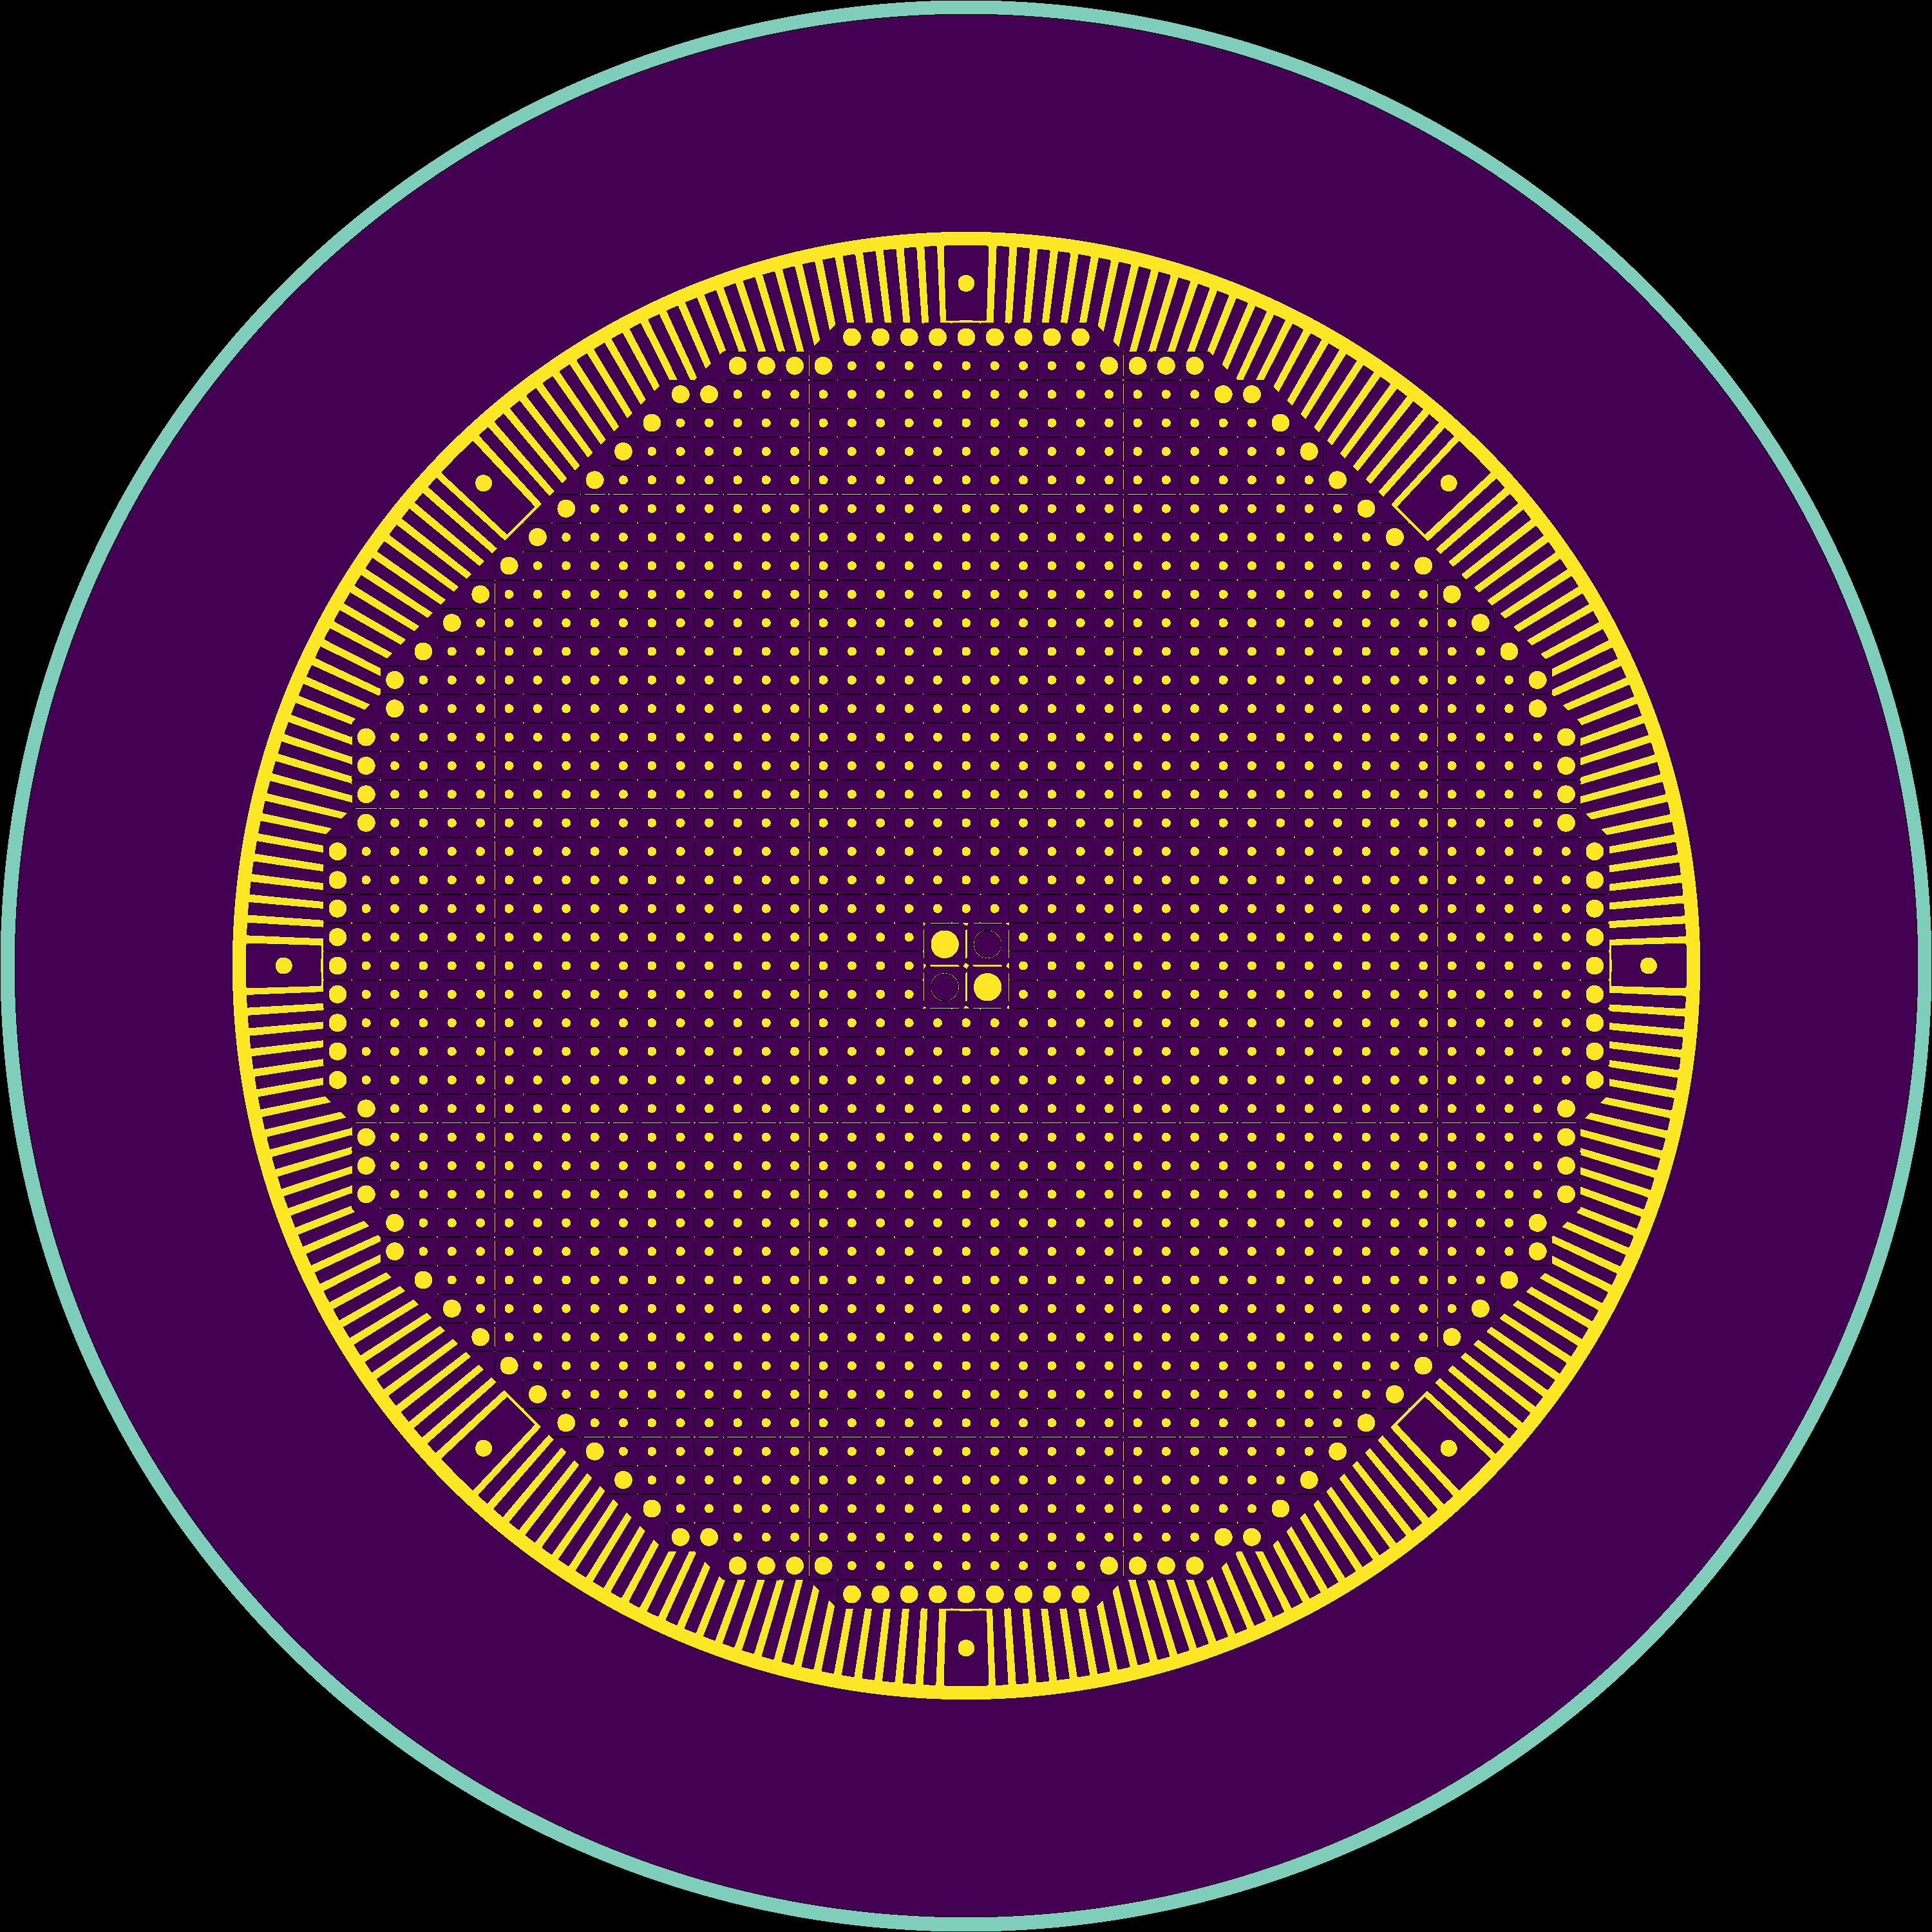
\includegraphics[width=\linewidth]{figure_2_1.png}
  \caption{Plan view of molten salt breeder reactor (MSBR) core.}
  \label{fig:plan}
\end{figure}

\begin{figure}[ht] % replace 't' with 'b' to force it to be on the bottom
  \centering
  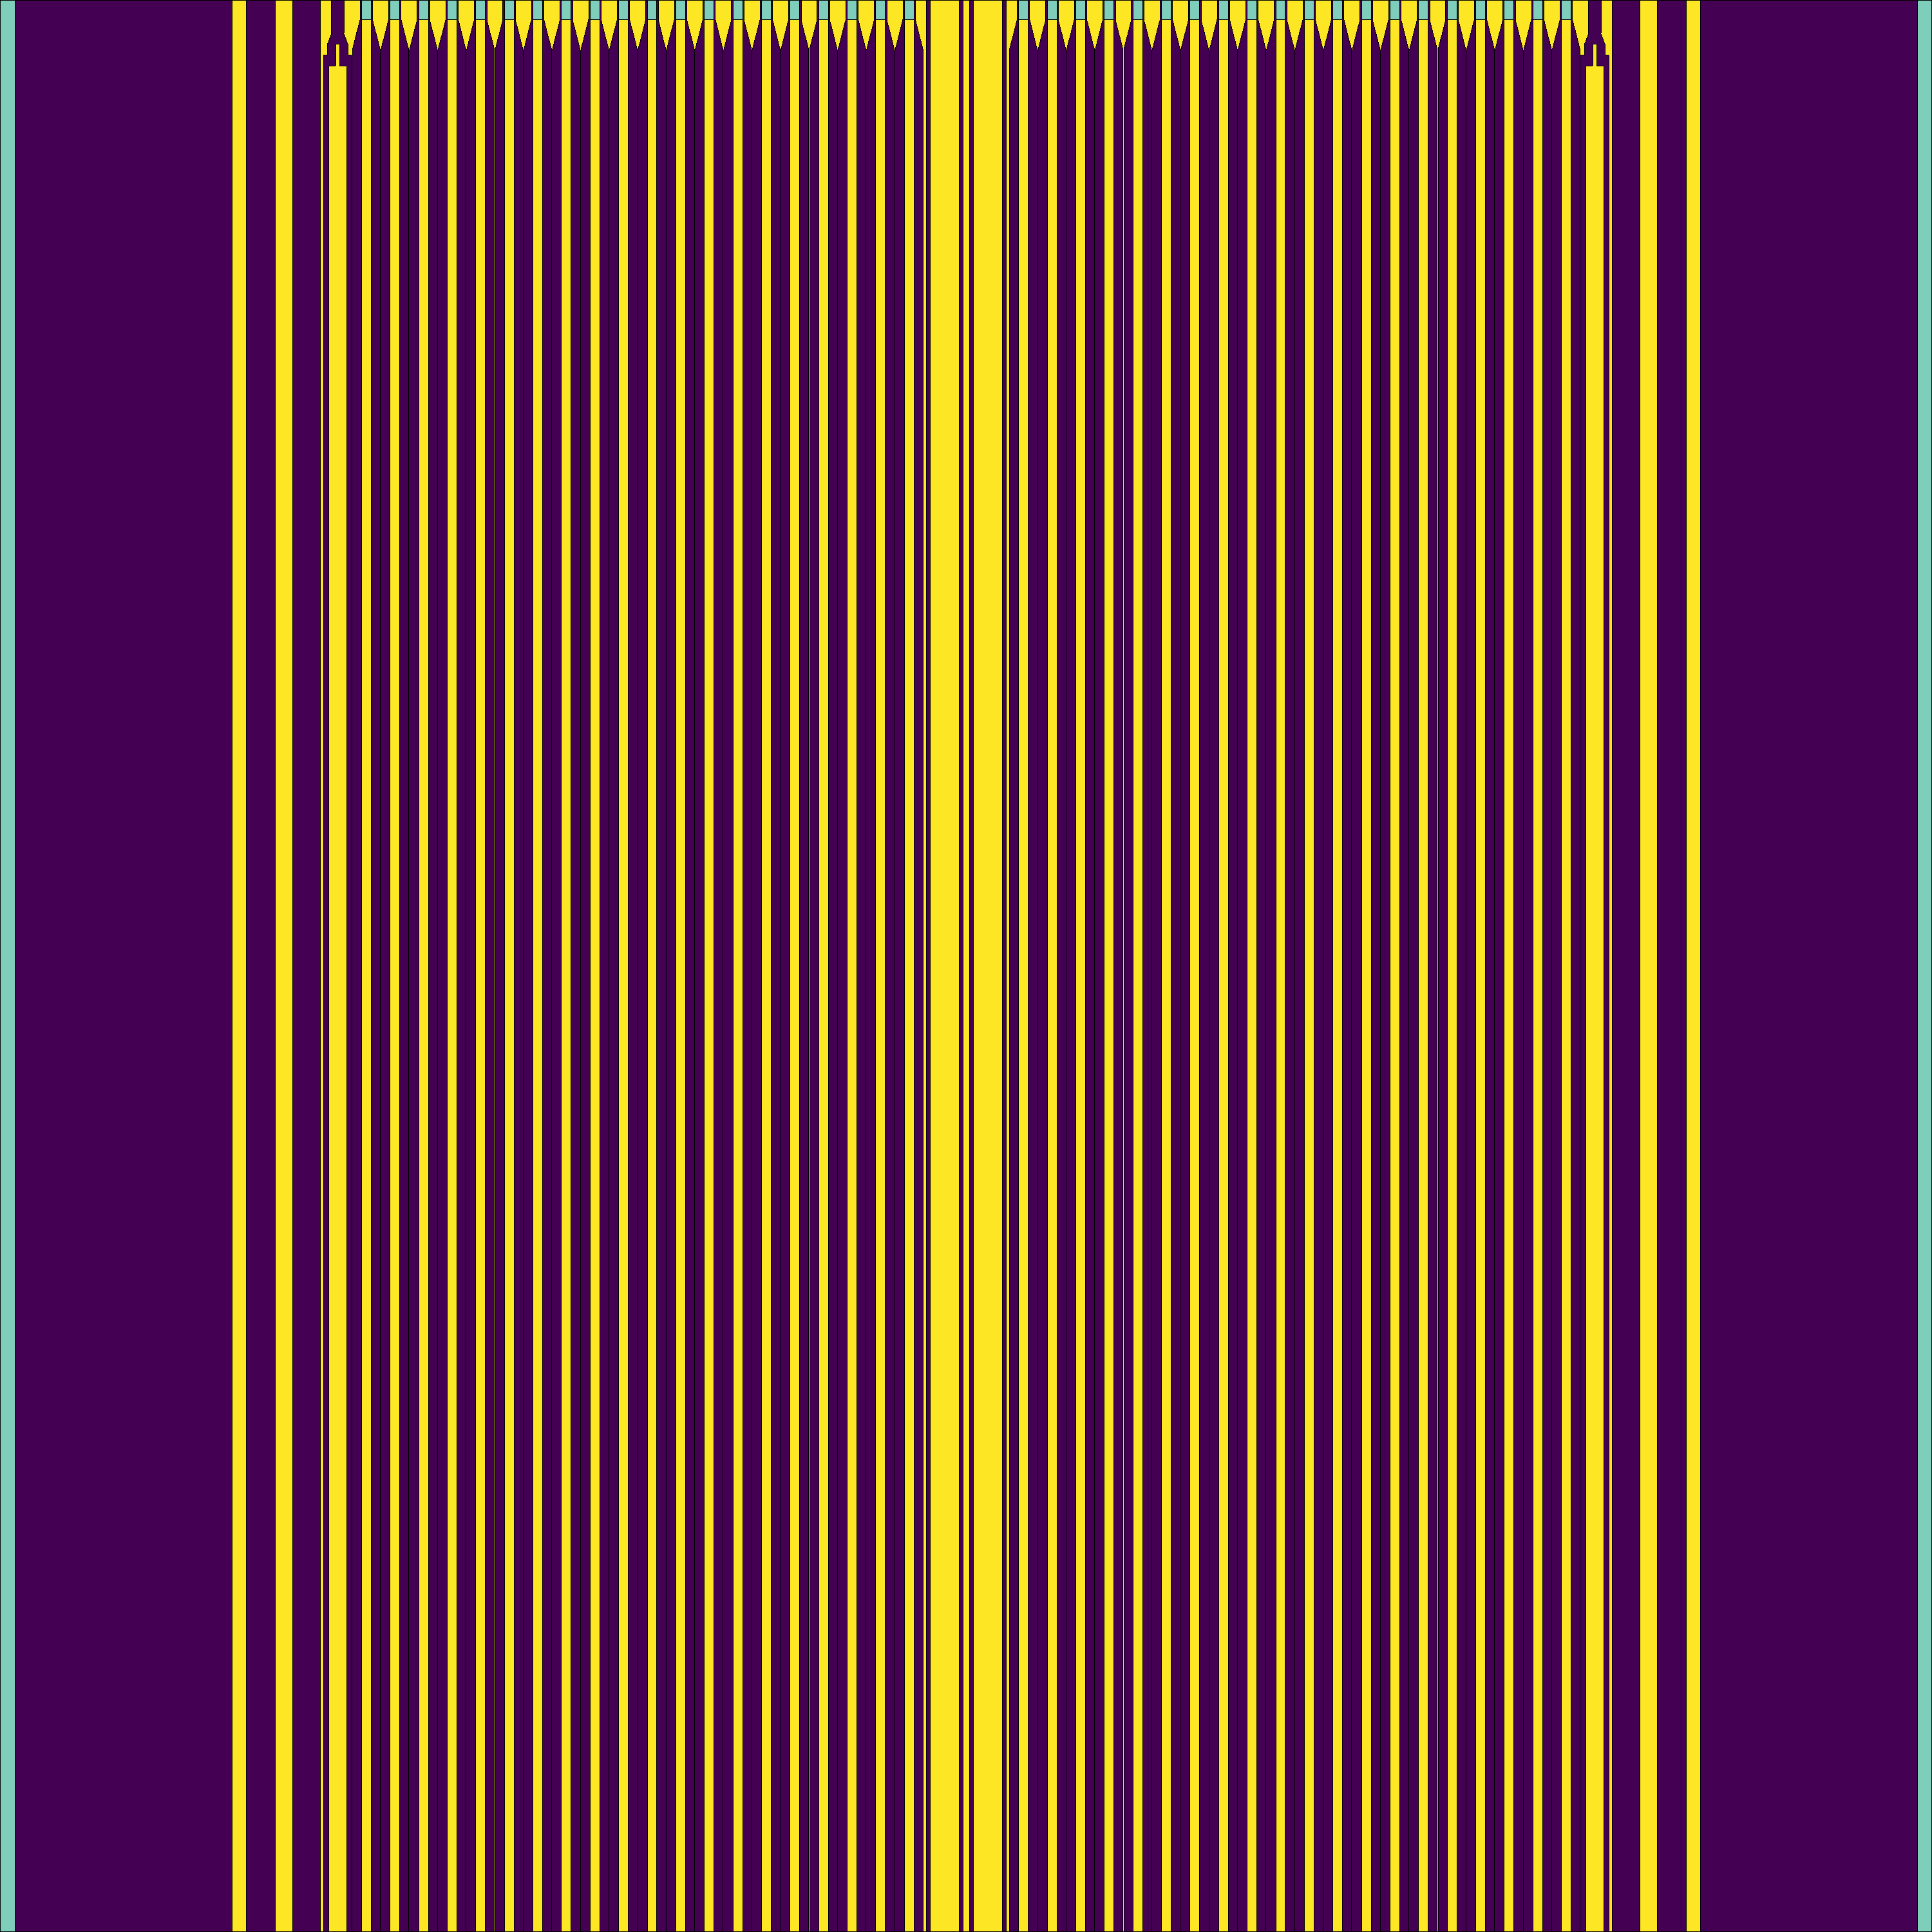
\includegraphics[width=\linewidth]{figure_2_2.png}
  \caption{Elevation view of molten salt breeder reactor (MSBR).}
  \label{fig:elevation}
\end{figure}

\subsection{2.1. Core zone I and II-A}
The central portion, called Zone I, is made up of $10.16cm\times10.16cm\times396.24cm$-long graphite elements. The fuel salt to graphite volume ratio of Zone 1 is 13.2\% which possible with a central hole diameter about $3.42cm$. Zone II having 37\% salt and central hole diameter about $6.604cm$. Both types of elements mostly have a rectangular shape with a part of cylinder sticking out at each corner to form salt flow between the graphite channels. Different sizes of elements necessarily to reduce the peak damage flux and power density in the center of the core to prevent local graphite damage. Figure~\ref{fig:zone12A} demonstrates the reconstructed graphite element utilized for Serpent model.

\begin{figure}[h] % replace 't' with 'b' to force it to be on the bottom
  \centering
  
\includegraphics[width=0.96\linewidth]{figure_2_4.png}
  \caption{Zone I (left) and Zone II-A (right) elements.}
  \label{fig:zone12A}
\end{figure}

\subsection{2.2. Core zone II-B}
Second core zone is divided into two different zones: Zone II-A and Zone II-B. The graphite elements for zone II-A are prismatic and form first reflecting layer surrounding the core zone I. The elements for zone II-B made up in the form of rectangular slats spaced far enough apart to achieve 0.37 fuel salt volume fraction. Figure~\ref{fig:zone2B} shows Zone II, 5.08cm-wide annular space between the core graphite and the radial reflector graphite. The annulus contains 100\% fuel salt and serves to reduce the damage flux for internal surface of the graphite reflector blocks. From the ORNL report suggested model for Zone II-B has 8 graphite elements every $45^\circ$ with special shape and have holes for the flow of salt and were simplified into a uniformly sized chopped fan shape with the central hole. All other graphite $5.08cm$-thick slats and various length in width (average width is about $26.67cm$ are reconstructed as is in the model without any approximation. 

\subsection{2.3. Material composition}
The fuel salt, the reactor graphite, and the modified Hastelloy N are exclusive MSBR materials which have been created at ORNL for a program which have been started over 15 years ago. The isotope composition of each material at the initial state was detailed described in the MSBR conceptual design study \cite{robertson_conceptual_1971} and have been applied to Serpent model without any modification. 

\begin{figure}[hb] % replace 't' with 'b' to force it to be on the bottom
  \centering
  
\includegraphics[width=0.93\linewidth]{figure_2_5.png}
  \caption{Plan view of Zone II-B.}
  \label{fig:zone2B}
\end{figure}

Initial fuel salt loading composition is $LiF-BeF_2-ThF_4-^{233}UF_4-^{239}PuF_3$ (72-16-12-0.232-0.0006 mole \%). The lithium is enriched to 99.995\% $^{7}Li$ because $^{6}Li$ is a very strong neutron poison and becomes tritium. In this study, 0.005\% atomic fraction of $^{6}Li$ have been taken into account because even such a small amount of isotope with very high absorption cross section might significantly affect on effective multiplication factor. For cross section data generation ENDF/B-VII was employed \cite{chadwick_endf/b-vii.0:_2006}. %Specific temperature was fixed for each material to correctly model the Doppler-broadening of resonance peaks when Serpent generate problem-oriented nuclear data library.

%%%%%%%%%%%%%%%%%%%%%%%%%%%%%%%%%%%%%%%%%%%%%%%%%%%%%%%%%%%%%%%%%%%%%%%%%%%%%%%%
\section{3. Results and Analysis}
The reactor physics calculation was carried out using the methods described earlier. This section presenting calculation results, such as the effective multiplication factor for whole core, neutron flux spectrum, and temperature reactivity coefficients. The normalized neutron flux distribution is calculated for the whole core using continuous-energy nuclear data which allows to obtaining very smooth distribution. The temperature coefficients for both fuel salt solution and reactor graphite are computed by comparing effective multiplication factors for two temperatures in the working range.

The MSBR criticality simulations were performed on one Intel Xeon E3-1225 3.3GHz processor wich has four physical cores, each simulation takes 23 minutes or 92 minutes per one core. Similar whole-core MSBR simulation using MCNP6 required approximately 890 minutes per core \cite{park_whole_2015}, consequently, Serpent 2 can provide tremendous computer costs savings for heavy depletion computations.

\subsection{3.1. Neutron spectrum}
Figure~\ref{fig:spectrum} demonstrates the normalized neutron flux spectrum for the whole core in the energy range from $10^{-10}$ to $100 MeV$. The results shows close fit with the MCNP simulation \cite{park_whole_2015}, especially in thermal energy range. 
\begin{figure}[h!] % replace 't' with 'b' to force it to be on the bottom
  \centering
  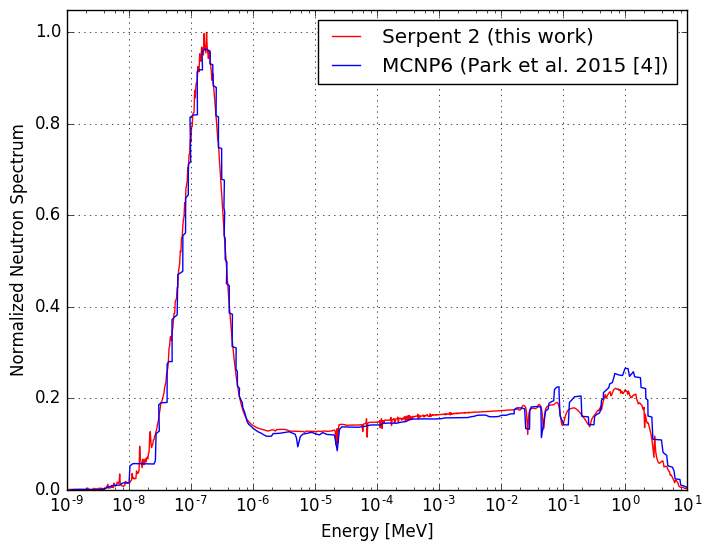
\includegraphics[width=\linewidth]{figure_3_1.png}
  \caption{Neutron flux spectrum of MSBR for MCNP6 and Serpent2 model.}
  \label{fig:spectrum}
\end{figure}
There is important to obtain epithermal or thermal spectrum to produce $^{233}U$ from $^{232}Th$ because radiative capture cross section of thorium monotonically decreasing from $10^{-10} MeV$ to $10^{-5} MeV$. Hardening the spectrim tends to significantly increasing resonance absorbtion in thorium and decreasing the absorptions in fissile and construction materials thus large amount of fissile material will be needed to make the reactor critical.

\subsection{3.2. Effective multiplication factor}
Table~\ref{tab:keff} shows the effective multiplication factor for both MCNP6 and Serpent2 whole core models. The coefficient obtained using Serpent2 is about 4.37\% higher than MCNP6 one. The discrepancy was ocurred most likely because Park and his colleagues didn't take into account $^{239}PuF_3$, contained in the fuel salt solution. Plutonium-239 has very high fission cross section in thermal energy range and produce more neutrons per fission than $^{233}U$, consequently, multiplication factor for this case is higher.
%%%%%%%%%%%%%%%%%%%%%%%%%%%%%%%%%%%%%%%%
\captionsetup[table]{
  labelsep = newline,
  name = TABLE, 
  justification=justified,
  singlelinecheck=false,%%%%%%% a single line is centered by default
  labelsep=colon,%%%%%%
  skip = \medskipamount}
\begin{table}[h!]
%\centering
\begin{tabular}{p{0.15\linewidth} p{0.3\linewidth} p{0.3\linewidth}} \toprule
      & Serpent2      & MCNP6 \cite{park_whole_2015}          
\\ \midrule
$K_{eff}$  & $1.05134\pm0.00116$ & $1.00736$
\\
\bottomrule
\end{tabular}
  \caption{Effective multiplication factor of whole core model.}
  \label{tab:keff}
\end{table}
%%%%%%%%%%%%%%%%%%%%%%%%%%%%%%%%%%%%%%%%%%%%%%%%%%%%%%%%%%%%%%%%%%%%%%%%%%%%%%%%
\subsection{3.3. Temperature effect of reactivity}
Table~\ref{tab:tcoef} represents the quantitive analysis of temperature effects on reactivity. Uncertainty for each temperature coefficient also was calculated and shown in Table~\ref{tab:tcoef}. Main physical principle underlies the reactor temperature feedback is expanding of a matter when it is heated. When fuel salt temperature increases, the density of the salt decreases, but at the same time, the total volume of fuel salt in the core remains constant because it is defined by the space for fuel in the graphite. When the reactor graphite temperature growing, the density of graphite declines which also free up space for fuel salt. To determine temperature coefficients three cases were considered:
\begin{enumerate}  
\item Temperature of fuel salt growing from 900K to 1200K.
\item Temperature of graphite increasing from 900K to 1200K. 
\item Whole reactor temperature rising from 900K to 1200K.
\end{enumerate}

%%%%%%%%%%%%%%%%%%%%%%%%%%%%%%%%%%%%%%%%
\captionsetup[table]{
  labelsep = newline,
  name = TABLE, 
  justification=justified,
  singlelinecheck=false,%%%%%%% a single line is centered by default
  labelsep=colon,%%%%%%
  skip = \medskipamount}
\begin{table}[h!]
%\centering
\begin{tabular}{p{0.22\linewidth} p{0.22\linewidth} p{0.21\linewidth} p{0.15\linewidth}} \toprule
   Reactivity coefficient [pcm/K]  & Serpent2      & MCNP6 \cite{park_whole_2015}   & Reference \cite{robertson_conceptual_1971}      
\\ \midrule
Fuel salt        & $-3.93\pm0.005$ & $-3.20\pm0.05$ & $-3.22$ 
\\ \midrule
Moderator        & $+2.44\pm0.013$ & $-0.11\pm0.05$ & $+2.35$ 
\\ \midrule
Total            & $-1.74\pm0.030$ & $-3.21\pm0.04$ & $-0.87$ 
\\
\bottomrule
\end{tabular}
  \caption{Temperature coefficient of reactivity.}
  \label{tab:tcoef}
\end{table}
%%%%%%%%%%%%%%%%%%%%%%%%%%%%%%%%%%%%%%%%%%%%%%%%%%%%%%%%%%%%%%%%%%%%%%%%%%%%%%%%
On the one hand, changes in fuel temperature cause only density variation, geometry keeps the same because fuel is in the form of liquid. On the other hand, when moderator heats up both the density and the geometry changes due to thermal expansion of the graphite blocks and the reflector. New graphite density was calculated using linear temperature expansion coefficient of reactor graphite which is $1.3\times10^{-6}1/K$ \cite{robertson_conceptual_1971}. Based on this information new geometry input, which takes into account graphite expansion, was created.

The fuel temperature coefficient (FTC) is positive due to thermal Doppler broadening of the resonance capture cross sections in the thorium and is in a good agreement with early research \cite{robertson_conceptual_1971,park_whole_2015}. The moderator temperature coefficient is negative due to changing density, and would increasing when reactor operating because of spectrum hardening along the fuel depletion \cite{park_whole_2015}. Finally, the total temperature coefficient of reactivity is relatively large negative, despite graphite component, and affords adequate reactor stability and controllability.
%%%%%%%%%%%%%%%%%%%%%%%%%%%%%%%%%%%%%%%%%%%%%%%%%%%%%%%%%%%%%%%%%%%%%%%%%%%%%%%%
\section{4. Conclusions}
The MSBR full-core analysis was performed using Monte Carlo code Serpent2. The complex geometry of the reactor is reconstructed in three-dimensional space without any major approximations. Accurate material data was employed to calculate reactor key design parameters. Effective multiplication factor for initial fuel composition is slightly higher than 1 (1.05) which allows reactor operates from startup to first online reprocessing cycle. The neutron flux energy spectrum was calculated for the whole core and represents the epithermal spectrum of the MSBR. The total temperature coefficient is negative, consequently, the MSBR has negative temperature feedback, but MTC is negative which is do not affect on safety because most of the energy releasing in the fuel salt.

The high-fidelity full-core model will be employed for a number of future works. First of all, depletion simulation will be performed using built-in Serpent 2 to find equilibrium state of the MSBR, optimal fuel salt composition, reprocessing characteristics (i.e. rates of removing fission products, the rate of adding thorium) and fuel utilization. Secondly, the model needed to generating problem-oriented nuclear data libraries for multi-physics models of MSRs developed in MOOSE-based coupled neutronics/thermal-hydraulics code Moltres \cite{lindsay_arfc/moltres:_2017}. Finally, transient accident simulations for safety investigation of the reactor core will be performed to studying the dynamic behavior of Molten Salt Breeder Reactor. 


%%%%%%%%%%%%%%%%%%%%%%%%%%%%%%%%%%%%%%%%%%%%%%%%%%%%%%%%%%%%%%%%%%%%%%%%%%%%%%%%
\bibliographystyle{ans}
\bibliography{bibliography}
\end{document}

